\documentclass{article}
\usepackage{amsmath}
\usepackage{amssymb}
\usepackage[svgnames]{xcolor}
\usepackage{graphicx}
\usepackage{enumitem}
\usepackage{multicol}
\usepackage{bbm}

\title{Computer Graphics: Assignment 06} % Title

\author{Lina Gundelwein, Letitia Parcalabescu, Anushalakshmi Manila} % Author name

\date{\today} % Date for the report

\begin{document}

\maketitle 

\section*{6.1 Bresenham Algorithm}
1. Rasterization
\begin{itemize}
\item First line initialization: 
\begin{align*}
& x_0 = 2 & x_1 = 6\\
& y_0 = 3 & y_1 = 4\\
& x = 2 & y = 3 \\
& d = F(3,3.5) = 3.5 \cdot 4 + 3\cdot(-1) + 8-18 =1\\
\end{align*}
\begin{enumerate}
\item color pixel $(x,y) = (2,3)$\\$d = 1 \geq 0 \Rightarrow E \rightarrow x = x+1 = 3,\, y = y = 3,\, d = d-1 = 0$
\item color pixel $(x,y) = (3,3)$\\$d = 0 \geq 0 \Rightarrow E \rightarrow x = x+1 = 4,\, y = y = 3,\, d = d-1 = -1$
\item color pixel $(x,y) = (4,3)$\\$d = -1 < 0 \Rightarrow NE \rightarrow x = x+1 = 5,\, y = y+1 = 4,\, d = d+3 = 2$
\item color pixel $(x,y) = (5,4)$\\$d = 2 \geq 0 \Rightarrow E \rightarrow x = x+1 = 6,\, y = y = 4,\, d = d-1 = 1$
\item color pixel $(x,y) = (6,4)$\\$d = 1 \geq 0 \Rightarrow E \rightarrow x = x+1 = 7,\, y = y = 4,\, d = d-1 = 0$
\end{enumerate}
\begin{figure}[htb]
\centering
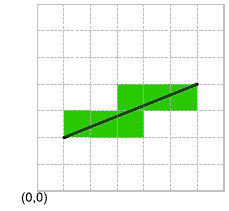
\includegraphics[width = 0.3\textwidth]{line1.png}
\end{figure}
\item Second line initialization, remember to switch x and y in the formulas: 
%\begin{align*}
%& x_0 = 3 & x_1 = 5\\
%& y_0 = 2 & y_1 = 5\\
%& x = 3 & y = 2 \\
%& d = F(4,2.5) =2.5 \cdot 2 + 4 \cdot(-3) +15-10 = -2\\
%\end{align*}
%\begin{enumerate}
%\item color pixel $(x,y) = (3,2)$\\$d = -2 < 0 \Rightarrow NE \rightarrow x = x+1 = 4,\, y = y+1 = 3,\, d = d-1 = -3$
%\item color pixel $(x,y) = (4,3)$\\$d = -3 < 0 \Rightarrow NE \rightarrow x = x+1 = 5,\, y = y = 4,\, d = d-1 = -4$
%\item color pixel $(x,y) = (5,4)$\\$d = -4 < 0 \Rightarrow NE \rightarrow x = x+1 = 6,\, y = y+1 = 5,\, d = d-1 = -5$
%\end{enumerate}
\end{itemize}

2. Antialiasing


\end{document}